% \DocumentMetadata{
%   pdfversion=2.0,
%   pdfstandard=ua-2,
%   testphase={phase-III,math,table,title}
% }

\documentclass[10pt, aspectratio=169, handout]{ltx-talk}
% https://www.texdev.net/ltx-talk/examples/
% ltx-presentation is the LaTeX3-based, accessibility-focused, modern alternative
% See: https://www.texdev.net/ltx-talk/examples/

% Accessibility and PDF/UA compliance
\usepackage[english]{babel}
\usepackage{fontspec} % modern font selection, enables unicode
\usepackage{unicode-math}
\usepackage{tagpdf}
\tagpdfsetup{activate-all,uncompress,interwordspace=true}
\usepackage{accsupp} % For accessibility
\usepackage{hyperref}
\hypersetup{
    colorlinks=true,
    linkcolor=blue,
    filecolor=magenta,      
    urlcolor=cyan,
    pdfapart=3,
    pdfa=true,
    pdfua=1,
    unicode=true,
    pdftitle={Introduction to Digital Signal Processing},
    pdfauthor={Maxx Seminario},
    pdfsubject={Digital Signal Processing: ECEN 463/863, Fall 2025},
    pdfkeywords={Signal Processing, Digital, Accessibility, Course, Slides},
    pdfcreator={XeLaTeX with ltx-presentation}
}

% Color contrast for accessibility
\usepackage{xcolor}
\definecolor{UNLRed}{RGB}{186,12,47}
\definecolor{UNLGray}{RGB}{88,89,91}
\definecolor{UNLBlue}{RGB}{0,46,93}
\colorlet{structurecolor}{UNLRed!80!black}

% Set font for readability
\setmainfont{Arial}
\setsansfont{Arial}
\setmonofont{Fira Mono}
\setmathfont{Latin Modern Math}

% For accessible figures and tables
\usepackage{graphicx}
\usepackage{caption}
\captionsetup{labelformat=empty, font=small, textfont=it, singlelinecheck=false}
\usepackage{subcaption}
\usepackage{tikz}
\usepackage{pgfplots}
\pgfplotsset{compat=newest}

\usepackage{amsfonts}
\usepackage{amsmath}
\usepackage{bm}
\usepackage{array}
\usepackage{makecell}
\usepackage{verbatim}

% Accessible tables
\usepackage{tabularx}
\usepackage{booktabs}

% Title metadata
\title{Introduction to Digital Signal Processing}
\subtitle{ECEN 463/863}
\author{Maxx Seminario}
\institute{University of Nebraska-Lincoln}
\date{August 25, 2025}

\begin{document}

\maketitle

\section{Introduction}

\begin{slide}{Teaching Staff}
\begin{block}{Instructor}
	\textbf{Maxx Seminario} \\
	Office hours: Mondays 2:30 -- 3:30 PM, SEC C215, or by appointment. \\
	e-mail: mseminario2@huskers.unl.edu
\end{block}
% \begin{block}{Teaching Assistant}
% 	\textbf{TBD} \\
% 	Office hours: TBD \\
% 	e-mail: TBD
% \end{block}
\end{slide}

\begin{slide}{Sources and Acknowledgments}
\begin{block}{Primary Sources}
\begin{itemize}
    \item \textbf{Textbook:} \emph{Discrete-Time Signal Processing}, Oppenheim and Schafer, 3rd Edition
    \item \textbf{UNL Digital Signal Processing Archive} (e.g., Prof. Michael Hoffman)
    \item \textbf{MIT Digital Signal Processing Course} (6.341/6.555J, Prof. Alan V. Oppenheim)
    \item \textbf{Stanford Digital Signal Processing Course} (EE264, Prof. Julius O. Smith III)
    \item \textbf{MIT OpenCourseWare (OCW)} \url{https://ocw.mit.edu/}
\end{itemize}
\end{block}
\end{slide}

\begin{slide}{Why \textbf{Digital} Signal Processing?}
\begin{itemize}
  \item Flexibility
  \item Accuracy
  \item Multi-purpose hardware
  \item Easy to implement sophisticated operations
  \item Today we have tremendous computer power
\end{itemize}
\end{slide}

\begin{slide}{Why \textbf{Digital} Signal Processing?}
The development of low-cost and high-speed digital electronics paved the way for digital signal processing.
\vspace{0.5cm}

\begin{figure}
    \centering
    \includegraphics[width=0.2\textwidth, alt={First point contact transistor (1947)}]{figs/First_point_contact_transistor_1947.jpg}
    \includegraphics[width=0.25\textwidth, alt={First integrated circuit (1961)}]{figs/first_ic_1961.jpg}
    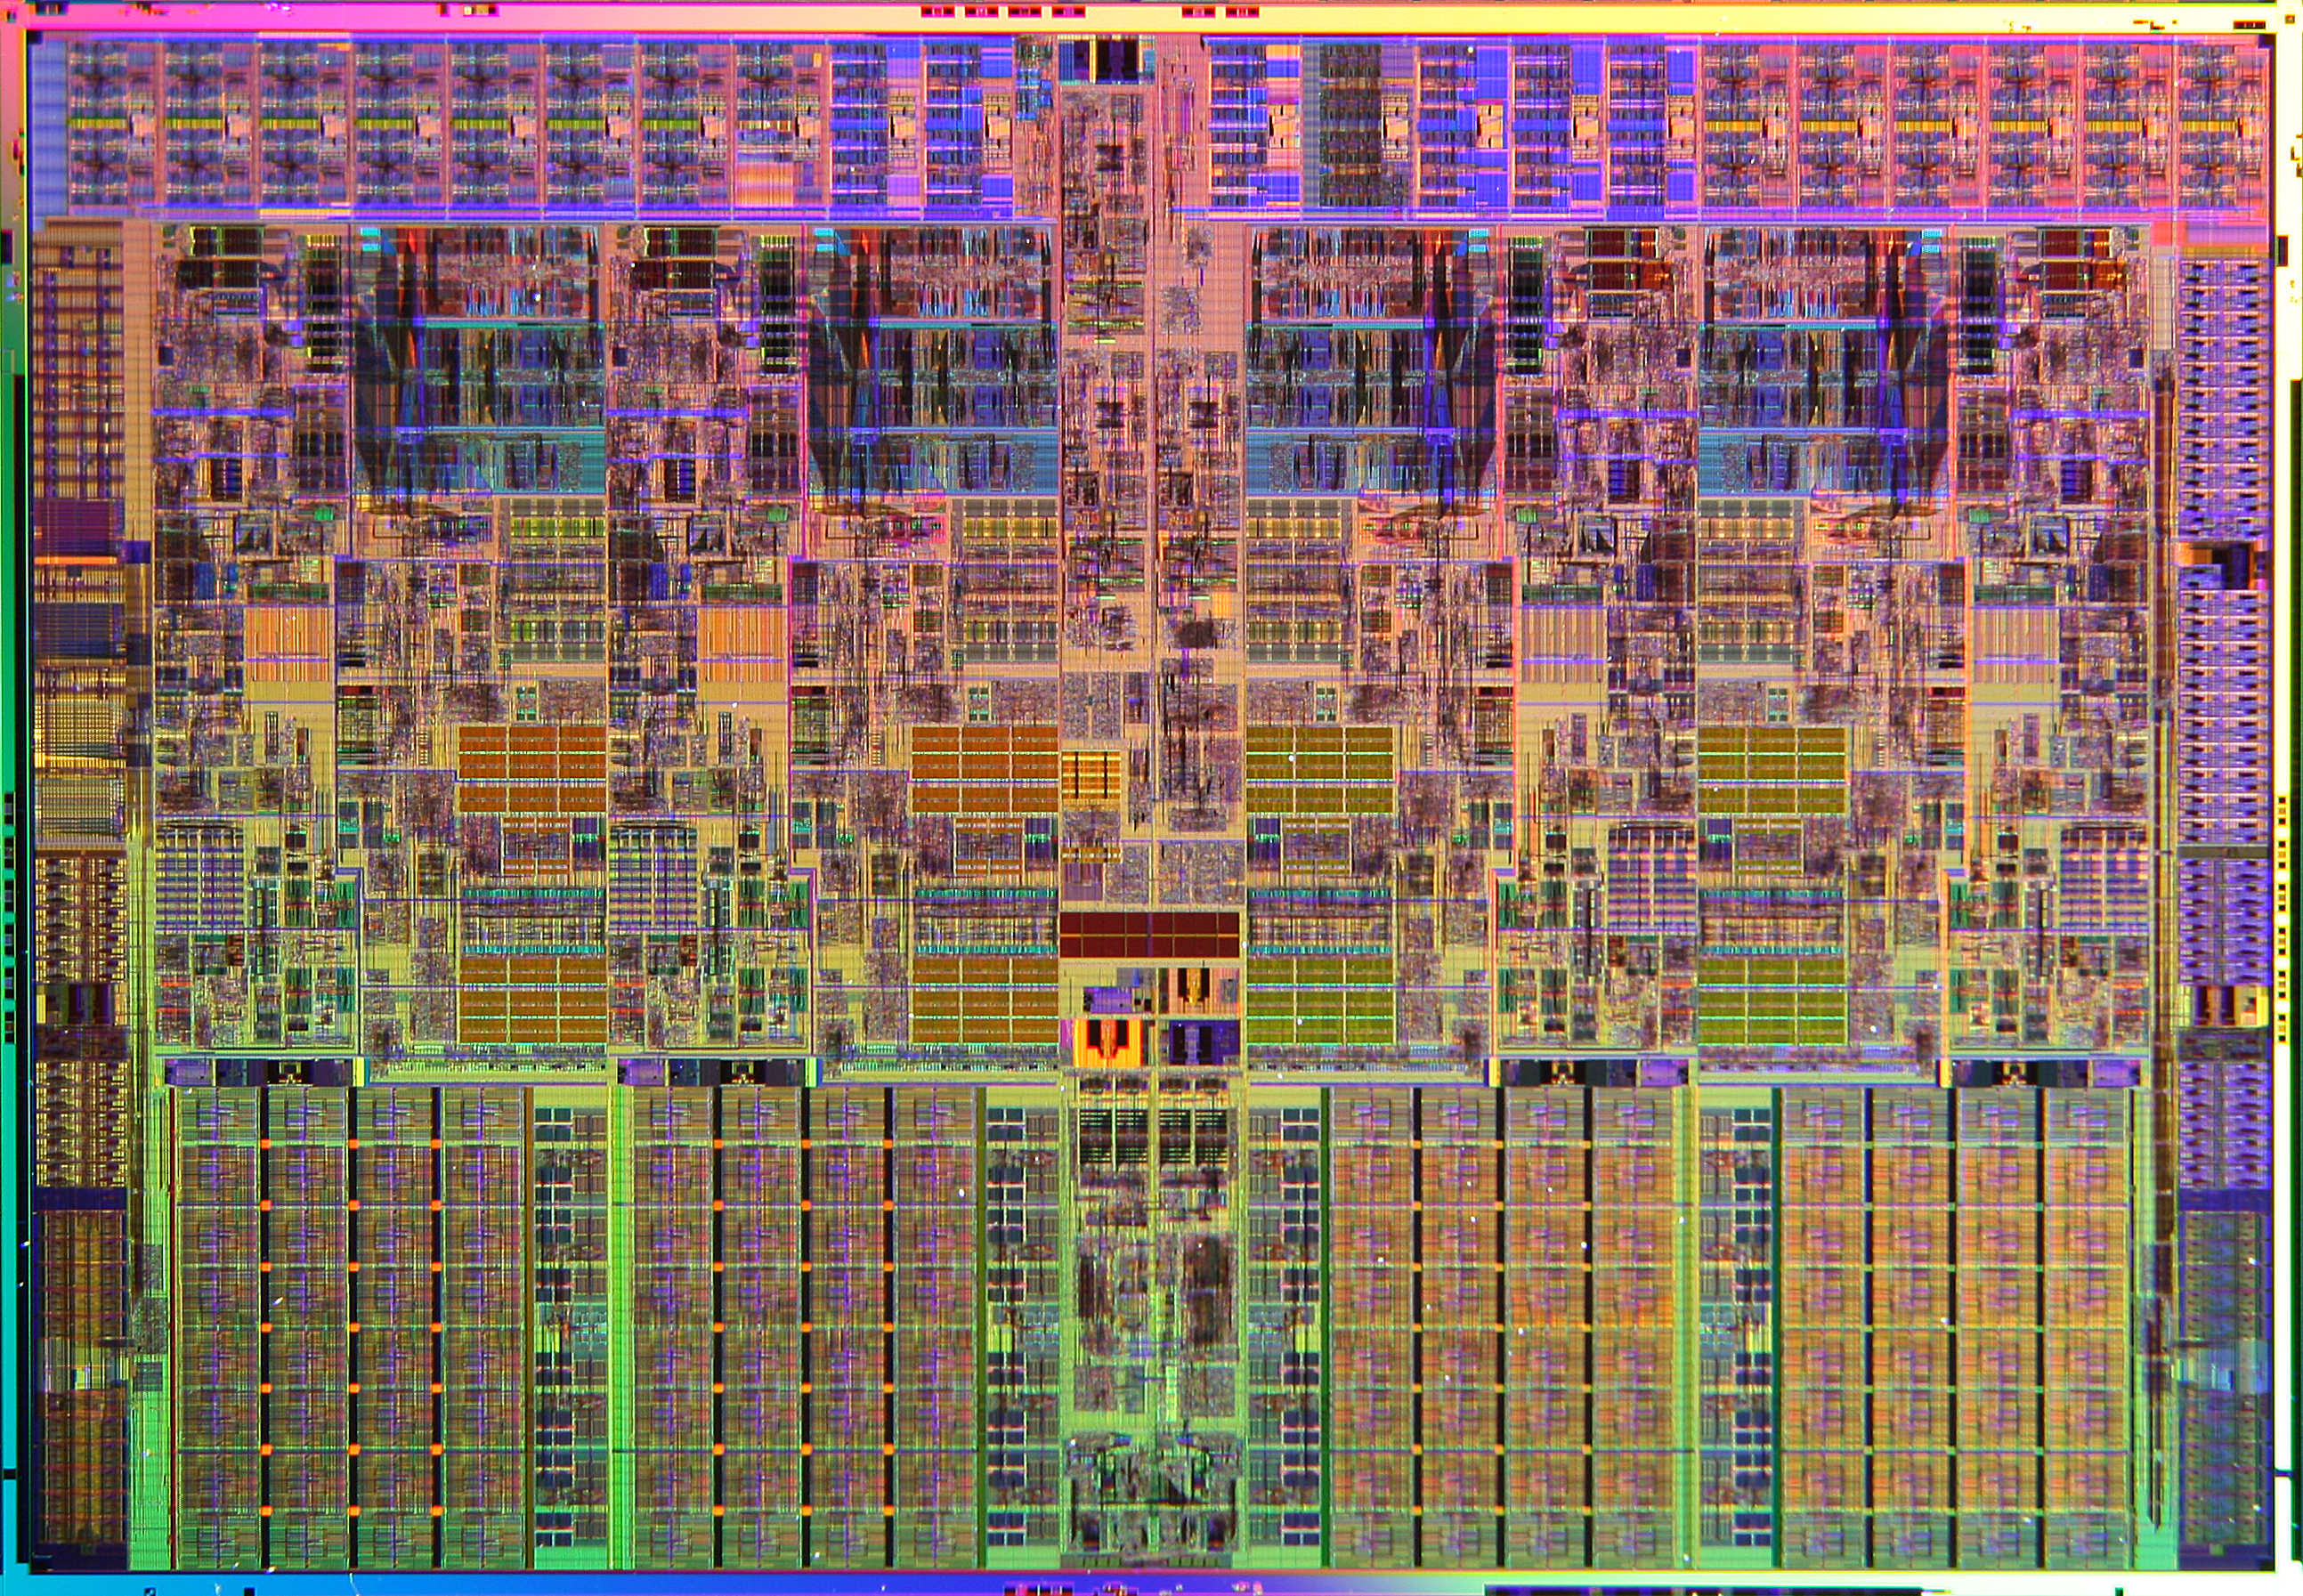
\includegraphics[width=0.2\textwidth, alt={Modern processor (200X)}]{figs/modern_i7.jpg}
    \caption{Evolution: First point contact transistor (1947), First integrated circuit (1961), Modern processor (200X)}
\end{figure}
\end{slide}

\begin{slide}{Why learn digital signal processing?}
\begin{itemize}
    \item Present in essentially all fields of modern EE
    \item Countless applications
\end{itemize}
\begin{figure}
    \centering
    \includegraphics[width=0.8\textwidth, alt={DSP and related areas}]{figs/ee264_and_related_areas.jpg}
    \caption{Applications of Digital Signal Processing in various areas}
\end{figure}
\end{slide}

\begin{slide}{Example: Digital Communication}
\begin{block}{Problem:}
    \begin{figure}
        \centering
        \includegraphics[width=0.5\textwidth, alt={Channel without equalization}]{figs/channel_no_eq.pdf}
        \caption{Channel without equalization}
    \end{figure}
\end{block}
\begin{block}{Solution:}
    \begin{figure}
        \centering
        \includegraphics[width=0.7\textwidth, alt={Channel with equalization}]{figs/channel_eq.pdf}
        \caption{Channel with equalization}
    \end{figure}
\end{block}
\end{slide}

\begin{slide}{Example: Speech Recognition}
\begin{figure}
    \centering
    \includegraphics[width=0.65\textwidth, alt={Speech spectrogram, 16 kHz sampling rate}]{figs/speech_spectogram.pdf}
    \caption{Spectrogram of a speech signal (16 kHz sampling rate)}
\end{figure}
\end{slide}

\begin{slide}{Example: Speech Recognition}
\begin{figure}
    \centering
    \includegraphics[width=0.65\textwidth, alt={Recurrent Neural Network for Speech Recognition}]{figs/recurrent_neural_net.pdf}
    \caption{Recurrent Neural Network for Speech Recognition}
\end{figure}
\end{slide}

\begin{slide}{Example: Speech Recognition}
Spectrogram of the same speech signal, now recorded with sampling rate of 44.1 kHz.
\vspace{0.5cm}
\begin{figure}
    \centering
    \includegraphics[width=0.7\textwidth, alt={Speech spectrogram, 44.1 kHz sampling rate}]{figs/speech_spectogram_44k.pdf}
    \caption{Spectrogram at 44.1 kHz sampling rate}
\end{figure}
More on spectrograms and short-time Fourier transform on lecture 11.
\end{slide}

\begin{slide}{Digital processing of analog signals}
\begin{figure}
    \centering
    \includegraphics[width=0.7\textwidth, alt={ADC-DSP-DAC Diagram}]{figs/adc-dsp-dac.pdf}
    \caption{Analog-to-Digital and Digital-to-Analog conversion in a DSP system}
\end{figure}
\begin{block}{Analog-to-digital converter (ADC)}
    \begin{itemize}
        \item Performs filtering, sampling, and quantization
        \item Sampling rate may be tens of kHz (audio) or tens of GHz (optical comms)
    \end{itemize}
\end{block}
\begin{block}{Digital signal processor}
    \begin{itemize}
        \item Performs operations such as filtering, FFT, etc.
        \item Can be implemented on PCs or ASICs
    \end{itemize}
\end{block}
\begin{block}{Digital-to-analog converter (DAC)}
    \begin{itemize}
        \item Performs quantization and reconstruction (filtering)
        \item Sampling rate could be similar to ADC
    \end{itemize}
\end{block}
\end{slide}

%%%%%%%%%%%%%%%%%%%%%%%%%
\section{Administrative}

\begin{slide}{Administrative: Resources}
\begin{block}{Textbook}
    \begin{itemize}
        \item ``Discrete-Time Signal Processing'', Oppenheim and Schafer, 3rd edition, 2010.
    \end{itemize}
    \begin{figure}
        \centering
        \includegraphics[width=0.15\textwidth, alt={Book cover}]{figs/book_cover.jpg}
    \end{figure}
\end{block}
\begin{block}{Lecture notes}
    \begin{itemize}
        \item Lecture notes will cover all material, but reading the textbook is encouraged.
    \end{itemize}
\end{block}
\begin{block}{Canvas: \href{https://canvas.unl.edu}{canvas.unl.edu}}
    \begin{itemize}
        \item Lecture notes, homework assignments, Matlab code.
        \item Submit homework on Canvas.
    \end{itemize}
\end{block}
\end{slide}

\begin{slide}{Administrative: Assignments}
\begin{itemize}
    \item Assignments released Friday, due next Friday at 11:59pm.
    \item Submit a single PDF with your solutions to Canvas.
    \item Homework includes analytical derivations and Matlab simulations.
    \item Discussion is encouraged, but submit your own work.
    \item No late submissions. Contact instructor for extensions in advance.
\end{itemize}
\end{slide}

\begin{slide}{Administrative: Grading}
\begin{itemize}
    \item Quizzes: $10\%$
    \item Homework Assignments: $30\%-60\%$
    \item Exams: $30\%-60\%$ (Based on 1 or 2 Exams)
\end{itemize}
\end{slide}

\begin{slide}{Administrative: Enrollment}
\begin{itemize}
    \item Deadline to drop for 100\% refund: September 2
    \item Last day to drop and remove from record: September 5
    \item 75\% refund: September 5
    \item 50\% refund: September 12
    \item 25\% refund: September 19
    \item Last day to change Pass/No Pass: October 17
    \item Withdrawals with “W” grade: November 14
\end{itemize}
\end{slide}

\end{document}